\documentclass[../relazione.tex]{subfiles}
\graphicspath{{\subfix{../images/}}}

\begin{document}
\section{Analisi delle prestazioni su diversi Device}
Riportiamo ora i tempi medi di runtime ottenuti eseguendo dei test con la versione \textit{Rectangular} su un dataset di 4096 elementi eseguito per 15 volte su ognuno dei seguenti dispositivi:
\begin{enumerate}
    \item NVIDIA CUDA GeForce GTX 1650 with Max-Q Design				
    \item Intel(R) UHD Graphics
    \item Intel(R) Core(TM) i7-10710U CPU @ 1.10GHz
\end{enumerate}

\subsection{Versione \textit{Rectangular}}
\begin{figure}[H]
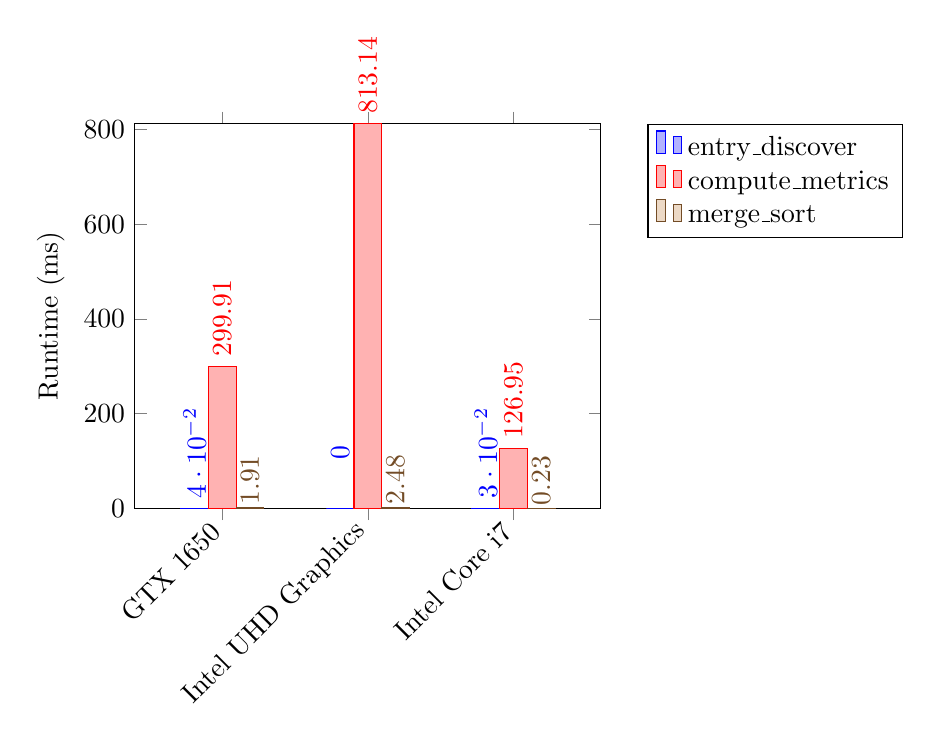
\begin{tikzpicture}
\begin{axis}[
symbolic x coords={
GTX 1650,
Intel UHD Graphics,
Intel Core i7
},
xtick=data,
x tick label style={rotate=45,anchor=east},
nodes near coords,
every node near coord/.append style={rotate=90, anchor=center},
ylabel=Runtime (ms),
legend style={at={(1.1, 0.85)}, anchor=west},
ybar=0pt,
legend cell align={left},
enlarge x limits=0.3,
enlarge y limits=0,
width=7.5cm,
]
\addplot+[every node near coord/.append style={yshift=10pt, xshift=30pt}] coordinates { %entries discover
(GTX 1650, 0.04)
(Intel UHD Graphics, 0.00)
(Intel Core i7, 0.03)
};
\addplot+[every node near coord/.append style={xshift=0pt, anchor=west}] coordinates { %compute metrics
(GTX 1650, 299.91)
(Intel UHD Graphics, 813.14)
(Intel Core i7, 126.95)
};
\addplot+[every node near coord/.append style={yshift=-10pt, xshift=0pt}] coordinates { %mergesort
(GTX 1650, 1.91)
(Intel UHD Graphics, 2.48)
(Intel Core i7, 0.23)
};
\legend{entry\_discover, compute\_metrics, merge\_sort}
\end{axis}
\end{tikzpicture}
\caption{Tempi di runtime della versione \textit{Rectangular}}
\end{figure}

\subsection{Versione \textit{Rectangular} vettorizzata}

\begin{figure}[H]
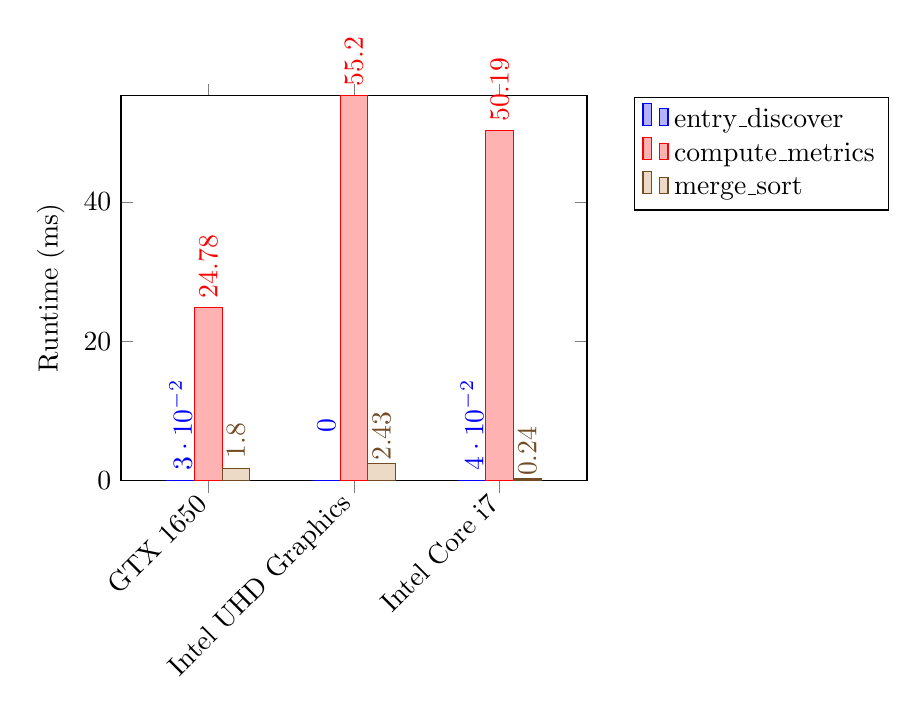
\begin{tikzpicture}
\begin{axis}[
symbolic x coords={
GTX 1650,
Intel UHD Graphics,
Intel Core i7
},
xtick=data,
x tick label style={rotate=45,anchor=east},
nodes near coords,
every node near coord/.append style={rotate=90, anchor=center},
ylabel=Runtime (ms),
legend style={at={(1.1, 0.85)}, anchor=west},
ybar=0pt,
legend cell align={left},
enlarge x limits=0.3,
enlarge y limits=0,
width=7.5cm,
]
\addplot+[every node near coord/.append style={yshift=10pt, xshift=30pt}] coordinates { %entries discover
(GTX 1650, 0.03)
(Intel UHD Graphics, 0.00)
(Intel Core i7, 0.04)
};
\addplot+[every node near coord/.append style={xshift=0pt, anchor=west}] coordinates { %compute metrics
(GTX 1650, 24.78)
(Intel UHD Graphics, 55.20)
(Intel Core i7, 50.19)
};
\addplot+[every node near coord/.append style={yshift=-10pt, xshift=0pt}] coordinates { %mergesort
(GTX 1650, 1.80)
(Intel UHD Graphics, 2.43)
(Intel Core i7, 0.24)
};
\legend{entry\_discover, compute\_metrics, merge\_sort}
\end{axis}
\end{tikzpicture}
\caption{Tempi di runtime della versione \textit{Rectangular} vettorizzata}
\end{figure}

\subsection{Confronto tra prestazioni attese e prestazioni effettive}
Tenendo conto dei dati teorici riguardanti la memory bandwidth delle varie piattaforme possiamo provare a determinare se questo algoritmo riesce effettivamente a sfruttare tutti i Device allo stesso modo oppure se qualcuno di questi performa meno di quanto dovrebbe.

In particolare le memorie dei Device su cui sono stati eseguiti i test hanno banda passante teorica pari a:
\begin{enumerate}
    \item Dedicata: 121.1 $GB/s$
    \item Integrata: 15.0 $GB/s$ (Dovuta al bus PCIe 3.0)
    \item CPU: 15.0 $GB/s$ (Dovuta al bus PCIe 3.0)
\end{enumerate}
da cui ne deriva una ratio pari a circa $16/3$ tra Dedicata e Integrata(o CPU).

I valori del test ottenuti con la versione \textit{Rectangular} vettorizzata mostrano invece una ratio di circa $20/9$, in sostanza la Dedicata performa meglio della Integrata(e della CPU) solo del doppio mentre i valori attesi vorrebbero la scheda Nvidia circa 5 volte più prestante della controparte.
Inoltre effettuando una modifica al codice, sfruttando cioè la funzione \lstinline{clEnqueueMapBuffer} fornita da OpenCL invece della precedente \lstinline{clEnqueueWriteBuffer}, le prestazioni della Intel UHD incrementano ulteriormente portando la ratio a circa $3/2$, cioè l'Integrata, potendo evitare i trasferimenti di dati con l'host visto che lavorano sulla stessa memoria, diventa solo di una volta e mezza più lenta della GPU integrata che ovviamente non può beneficiare di questa modifica.
La CPU invece sembra, stranamente, peggiorare i propri tempi di runtime in seguito a questa modifica.

Ne deduciamo che la GPU non è effettivamente sfruttata a pieno e che probabilmente le cause di questa mancanza sono da ricercare nella frammentazione della coda dei task da analizzare e nei trasferimenti di memoria con l'host necessari a terminare l'iterazione del kernel.

Il primo di questi problemi è dovuto al fatto che la coda, nella sua implementazione attuale, contiene un valore non nullo nelle posizioni dell'array che corrispondono ai nodi da analizzare. Per ovviare a questo problema si potrebbe pensare di usare una coda effettiva invece di un array, tuttavia questo non è possibile perché i workitem dovrebbero sincronizzarsi per decidere a quale indirizzo poter inserire il nuovo nodo da aggiungere alla coda.

Anche il secondo problema come discusso in precedenza non è risolvibile a causa dell'impossibilità di sincronizzare workitem di workgroup diversi.

\subsection{Andamento delle prestazioni}
Si riportano i risultati dei test eseguiti su una GPU NVIDIA GTX 1650 con dataset di varia grandezza. Per ogni dataset sono state eseguite 15 iterazioni con la versione \textit{Rectangular} vettorizzata dei kernel e successivamente sono stati calcolati i tempi medi di runtime:

\begin{center}
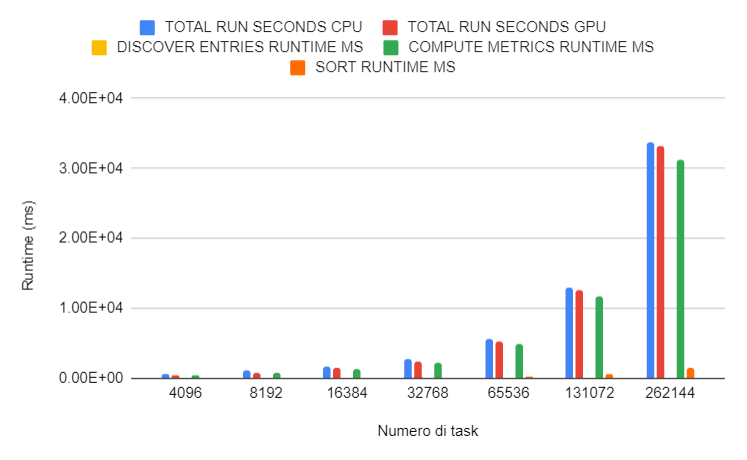
\includegraphics[scale=0.8]{images/andamento_prestazioni.png}
\end{center}

L'andamento delle prestazioni all'aumentare del numero di task è in linea con l'analisi asintotica presentata precedentemente. 

\end{document}